\chapter{Literature Review}
This work has conducted a literature review and existing tool exploration to 
identify problem that provide motivation for research. This chapter also presents a running example. The running example is used throughout this thesis to help introducing and explaining concepts, such as presenting related work (e.g. incrementality, state/change-based model persistence and comparison), explaining this work's proposed approaches to address the slow loading of change-based models, and discussing how change-based model persistence can be exploited to optimise model differencing and conflict detection.

\section{Running Example}
\label{sec:running_example_1}
Let's say that there is a project to develop a simplified class diagram model of a Role Playing Game (RPG). Jane, as the technical leader, set up the initial model (Fig. \ref{fig:class_diagram_origin}). She then assigned this work to Bob and Alice. Both of them continued to work on the model and made some modification producing the models in Figures \ref{fig:class_diagram_left} and \ref{fig:class_diagram_right} respectively.

\begin{figure}[ht]
  \begin{tabular}{l|c|r}
    \begin{subfigure}[t]{0.31\linewidth}
      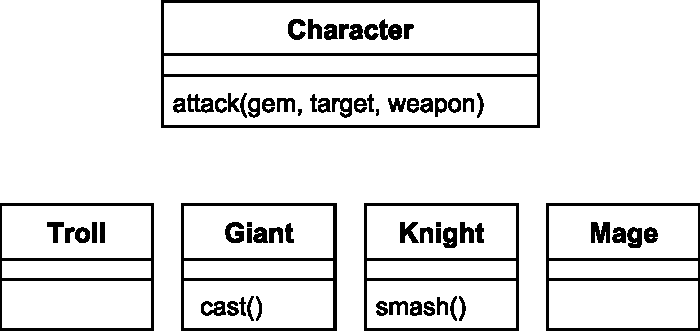
\includegraphics[width=\linewidth]{class_diagram_origin}
      \caption{original version (Jane's version)}
      \label{fig:class_diagram_origin}
    \end{subfigure}
    &
    \begin{subfigure}[t]{0.31\linewidth}
      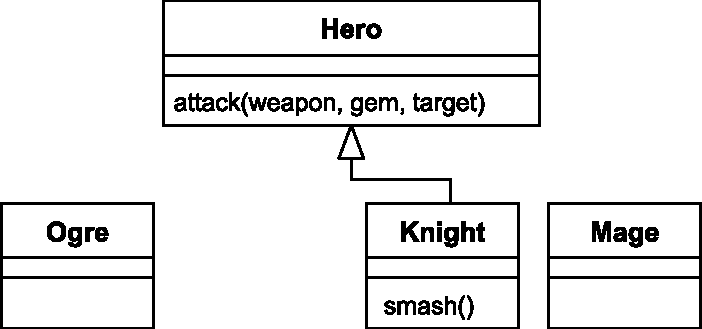
\includegraphics[width=\linewidth]{class_diagram_left}
      \caption{left version (Bob's version)}
      \label{fig:class_diagram_left}
    \end{subfigure}
    &
    \begin{subfigure}[t]{0.31\linewidth}
      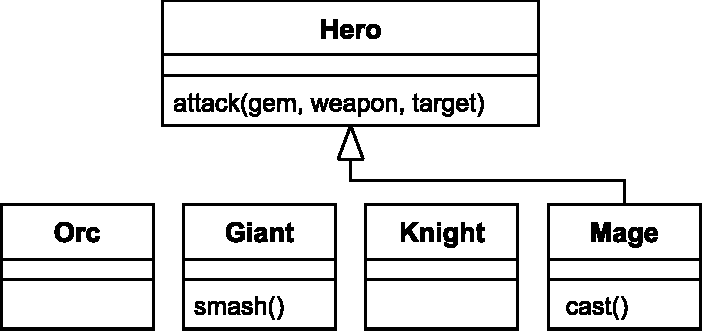
\includegraphics[width=\linewidth]{class_diagram_right}
      \caption{right version (Alice's version)}
      \label{fig:class_diagram_right}
    \end{subfigure}
  \end{tabular}
  \caption{Three class diagrams of a Role Playing Game.}
  \label{fig:class_diagram_rpg}
\end{figure}

The company where Jane, Bob, and Alice work applies incremental model management in their development process. Applying incrementality allows them to manage their models automatically based on every change made to their models. For example, validating names of classes against a naming convention or to updating a class' documentation when the class is modified. Implementing this incrementality also comes with challenge and it is discussed in Section \ref{sec:the_key_challenge_of_incrementality}.

\section{The Key-Challenge of Incrementality}
\label{sec:the_key_challenge_of_incrementality}
To illustrate the key-challenge of incrementality, I use the example in Fig. \ref{fig:class_diagram_rpg}. Let's say that after every modification to the model in Fig. \ref{fig:class_diagram_origin}, the model needs to be:

\begin{itemize}
  \item Validated against a naming convention that the name of a class should start with an uppercase.
  \item Transformed into a number of documentation files through a model-to-text transformation. Each class should have a documentation file.
\end{itemize}

Models in Figures \ref{fig:class_diagram_origin} and \ref{fig:class_diagram_left} are two consecutive versions. When the validation constraint is evaluated against the first version of the model (Fig. \ref{fig:class_diagram_origin}), it verifies that all the classes' names starts with a uppercase, and the model-to-text transformation then produces four documentation files that correspond to the classes in the model. In the sequel, in Fig. \ref{fig:class_diagram_left}, the model is updated by Bob. He applies several changes, such as renaming class \textsf{Character} to \textsf{Hero} and class \textsf{Troll} to \textsf{Ogre} and deleting class \textsf{Giant}.

A non-incremental model validation engine would treat the model of 
Fig. \ref{fig:class_diagram_left} as if it was a new model and would evaluate 
the constraint above against every class in the model. 
An incremental model validation engine, on the other hand, would identify 
that the previously established satisfaction of the constraint for classes 
\textsf{Knight} and \textsf{Mage} cannot have been possibly compromised by the changes made, and would only re-evaluate the constraint for classes \textsf{Character} and \textsf{Troll} (class \textsf{Giant} is deleted so it is not evaluated). 

Similarly, a non-incremental model-to-text transformation would generate 
and overwrite all documentation files. On the contrary, an 
incremental model-to-text transformation, would identify that it only needs to delete the documentation file of class \textsf{Giant} and generate documentation files for classes \textsf{Character} and \textsf{Troll} -- but not the documentation files of classes \textsf{Knight} and \textsf{Mage}, as these cannot have been affected by the changes made to the model.

While the overhead of executing transformations and validation constraints 
on small models like the one in Fig. \ref{fig:class_diagram_origin} is negligible, non-incremental execution can become a significant bottleneck for large evolving models. As stressed in Selic's seminal work \cite{selic2003pragmatics}, with reference to model-to-text transformation, ``... \textsf{this is particularly true in the latter phases of the development cycle when programmers make many small changes as they fine-tune the system. To keep this overhead low, it is crucial for the code generators to have sophisticated change impact analysis capabilities that minimize the amount of code regeneration}''.

As demonstrated by the pioneering work of Egyed \cite{egyed2011automatically}, 
to achieve incremental re-execution of (deterministic) queries on 
structured models, an execution engine needs to:

\begin{enumerate}
  \item Record model element property accesses during the initial execution of the queries;
  \item Identify new and deleted elements and modified model element properties in the new version of the model;
  \item Combine the information collected in the steps above to identify the subset of (potentially) affected rules/queries/templates that need to be re-executed.
\end{enumerate}

To illustrate this, this example uses an OCL implementation of the domain-specific constraint in List. \ref{lst:constraint}.

\begin{lstlisting}[style=ocl,caption={OCL constraint requiring that a class should start with an uppercase.},label=lst:constraint]
context Class
inv UpperCase: self.name->subtring(1, 1) == self.name->subtring(1, 1)->toUpper()
\end{lstlisting}

\begin{table}[ht]
  \centering
  \caption{Property-access trace of the evaluation of the constraint in List. \ref{lst:constraint} on the model of Fig. \ref{fig:class_diagram_origin}.}
  \begin{tabular}{p{4cm} p{2.1cm} p{2cm} p{2.1cm}}
    \hline 
    \textbf{Constraint} & \textbf{Context} & \textbf{Accessed Element} & \textbf{Accessed Property} \\ 
    \hline 
    \textsf{Class.UpperCase}  & \textsf{character} & \textsf{character} & \textsf{name} \\ 
    \textsf{Class.UpperCase}  & \textsf{troll} & \textsf{troll} & \textsf{name} \\ 
    \textsf{Class.UpperCase}  & \textsf{giant} & \textsf{giant} & \textsf{name} \\ 
    \textsf{Class.UpperCase}  & \textsf{knight} & \textsf{knight} & \textsf{name} \\
    \textsf{Class.UpperCase}  & \textsf{mage} & \textsf{mage} & \textsf{name} \\
    \hline 
  \end{tabular} 
  \label{tab:property_access_trace}
\end{table}

During the initial evaluation of the constraint on the model of Fig. \ref{fig:class_diagram_origin}, an incremental OCL engine would compute the property access trace displayed in Table \ref{tab:property_access_trace} as a side-product. Now, when the model is updated (Fig. \ref{fig:class_diagram_left}), the execution engine can identify that:

\begin{itemize}
  \item There is an element deleted in the model (class \textsf{Giant}) for which the constraint is not necessary to be evaluated;
  \item The value of property \textsf{name} of classes \textsf{Character} and \textsf{Troll} have changed, and as such, the constrain needs to be re-evaluated on this elements.
\end{itemize}

Egyed has shown that the property-access recording approach is applicable to queries of arbitrary complexity, 
as long as they are deterministic. More recent work has shown that variants of this approach can be used to 
achieve incrementality in a wide range of model processing operations, including model-to-model 
transformation \cite{jouault2010towards}, model-to-text transformation \cite{DBLP:conf/ecmdafa/OgunyomiRK15}, 
model validation, and pattern matching \cite{DBLP:conf/ecmdafa/RathHV12}---as long as changes to models can be 
precisely identified (step 2 in the list above).

\section{Identifying Changes in Models}
\label{sec:identifying_changes_in models}
There are two approaches in the literature for identifying changes in models 
in order to enable incremental re-execution of model processing operations.

\textbf{Notifications}. In this approach, the incremental execution 
engine needs to hook into the notification facilities 
provided by the modelling tool through which the developer edits the model, 
so that the engine can directly receive notifications as soon as 
changes happen (e.g. class \textsf{giant} has been deleted, class \textsf{character} has been renamed to ``Hero''). 
This is an approach taken by the IncQuery incremental pattern matching 
framework \cite{DBLP:conf/ecmdafa/RathHV12} and the ReactiveATL incremental model-to-model 
transformation engine \cite{DBLP:conf/ecmdafa/OgunyomiRK15}. The main advantage of this 
approach is that precise and fine-grained change notifications are provided 
for free by the modelling tool (and thus do not need to be computed by the 
execution engine---which as discussed below can be expensive and inefficient). 
On the downside, this approach is a poor fit for collaborative development 
settings where modelling and automated model processing activities are 
performed by different members of the team.

\textbf{Model Differencing}. This approach eliminates the coupling between 
modelling tools and incremental execution engines. Instead of depending on 
live notifications, in this approach the developer in charge of automated model 
processing, needs to have access to a copy of the last version of the model that the model processing program (e.g. the model-to-text transformation) was 
executed upon, so that it can be compared against the current version of 
the model (e.g. using a model-differencing framework such as SiDiff or 
EMFCompare) and the delta can be computed on demand. The main advantage of 
this approach is that it works well in a collaborative development environment 
where typically developers have distinct roles and responsibilities. On the 
downside, model comparison and differencing are computationally expensive and 
memory-greedy (both versions of the model need to be loaded into memory before 
they can be compared), thus largely undermining the time and resource saving 
potentials of incremental re-execution. 

In summary, incremental model processing currently delivers significant 
performance benefits only in a single-developer environment where the modeller 
is also responsible for performing all the (incremental) model processing 
operations. As a result, in collaborative development environments, 
developers need to either forgo incremental model processing altogether 
or to work around this limitation by manually steering model processing 
programs to process only subsets of their models, which is cumbersome and 
error prone.

\section{A Novel Solution to Incrementality}
\label{sec:a_novel_solution_to_incrementality}
A novel solution to incrementality should be able to deliver the advantages of both notification and model differencing approaches while eliminate their drawbacks. To realize such solution, this work comes with an idea that models can be persisted in their complete history of changes, a.k.a. change-based model persistence, as opposed to state-based model persistence that persists models in their snapshots at a time. In change-based model persistence, information about changes that have been applied to models can be preserved, and the persistence can be shared across the members of a team, for example through Version Control Systems (e.g., SVN, Git).The proposed change-based model persistence is discussed later in Chapter \ref{ch:change_based_model_persitence}. 

Moreover, change-based model persistence also can be exploited to optimise model comparison to only compares versions of a model on parts that have only been changed since their last shared common version. In other words, not every element of the versions is compared which can lead to a faster model comparison. This solution is discussed later in Chapters \ref{ch:model_differencing} and \ref{ch:conflict_detection}. 

\section{Change vs. State-based Persistence}
\label{sec:change_based_vs_state_based_persistence}
The concept of change-based persistence is not new and has been used in persisting changes of software, object-oriented databases, hierarchical documents, and models 
\cite{DBLP:journals/entcs/RobbesL07,DBLP:conf/sde/LippeO92,DBLP:conf/caise/IgnatN05,koegel2010emfstore}. 

The nature of change-based persistence give us two advantages. First, it contains finer-granularity information (e.g. types of changes, the order of the changes, elements that were changed, previous values, etc.) of changes which can improve the accuracy of change detection \cite{DBLP:journals/entcs/RobbesL07,DBLP:conf/sde/LippeO92,DBLP:conf/caise/IgnatN05,mens2002state}. Second, it records changes ordered manner which means that changes made to a model can be identified sequentially without having to explore and compare all elements of compared versions of models \cite{DBLP:conf/edoc/KoegelHLHD10}. The advantages to detect changes more precisely and much faster can then have positive knock-on effects on supporting (1) developers compare and merge models in collaborative modelling environments \cite{DBLP:conf/sde/LippeO92,DBLP:conf/caise/IgnatN05,koegel2010emfstore}, and (2) incremental model management \cite{jouault2010towards,DBLP:conf/ecmdafa/OgunyomiRK15, DBLP:conf/ecmdafa/RathHV12}. Moreover, changed-based persistence contains abundant information which can be exploited for analytics \cite{DBLP:journals/entcs/RobbesL07}.


Nevertheless, change-based persistence also comes with downsides, such as ever-growing model files 
\cite{DBLP:journals/entcs/RobbesL07,DBLP:conf/edoc/KoegelHLHD10} and increased model loading time \cite{mens2002state}
which increase storage and computation costs. A model that is frequently modified will increase considerably in file size 
since every change is added to the file. The increased file size (proportional to the number of persisted changes) will, 
in turn, increase the loading time of the model since all changes have to be replayed to reconstruct the model's 
eventual state. 

These downsides have to be mitigated to enable the practical adoption of change-based persistence. 
One approach to reducing the file size of change-based models is by removing changes that do not affect the eventual 
state of the model. For the increased loading time, it can be mitigated by ignoring -- i.e. not replaying -- changes 
that are cancelled out by later changes or employing change-based and state-based persistence side-by-side so that the
benefits of state-based persistence on loading time can be obtained. 

Other downsides are change-based persistence requires 
integration with existing tools -- since it is still a non-standard approach -- for its adoption \cite{koegel2010emfstore}, 
and still has limited support for standard, text-based version controls for collaborative development \cite{koegel2010emfstore}. 
These downsides can be addressed by developing a change-based persistence plugin for a specific development environment 
(e.g. Eclipse) and persisting changes in text-based format to support text-based version controls (e.g. Git, SVN).

%3-layer metamodelling architectures such as EMF and MOF. 
\begin{table}[t!]
    \centering
    \caption{The advantages and downsides between change-based and state-based persistence.}
    \label{table:advantages_drawbacks}
    \begin{tabular}
        {|>{\centering\arraybackslash}p{1.1cm}|>{\centering\arraybackslash}p{1.1cm}|>{\centering\arraybackslash}p{5cm}|>{\centering\arraybackslash}p{5cm}|}
        \hline 
        \multicolumn{2}{|c|}{\textbf{Dimensions}}&\textbf{Change-based Approach}&\textbf{State-based Approach}\\
        \hline 
        \multicolumn{2}{|p{2.2cm}|}{\centering Advantages} &
        \begin{minipage}[t]{5cm}
            \raggedright
            \begin{itemize}[leftmargin=9pt]
                \setlength\itemsep{2pt}
                \item[-] Faster for detecting changes \cite{DBLP:conf/edoc/KoegelHLHD10}
                \item[-] More accurate, carry semantic information \cite{DBLP:journals/entcs/RobbesL07,DBLP:conf/sde/LippeO92,DBLP:conf/caise/IgnatN05,mens2002state}  
                \item[-] Faster and more accurate for comparison and merging \cite{DBLP:conf/sde/LippeO92,DBLP:conf/caise/IgnatN05,koegel2010emfstore}
                \item[-] Information carried is useful for analytics \cite{DBLP:journals/entcs/RobbesL07}
            \end{itemize}
        \end{minipage}
        & 
        \begin{minipage}[t]{5cm}
            \raggedright
            \begin{itemize}[leftmargin=9pt]
                \setlength\itemsep{2pt}
                \item[-] Faster for loading large models \cite{DBLP:conf/models/Espinazo-PaganCM11,daniel2016neoemf,eclipse2019cdo}
                \item[-] A default standard, no need integration with existing tools \cite{koegel2010emfstore}  
            \end{itemize}
        \end{minipage}
        \\
        \hline
        \multicolumn{2}{|p{2.2cm}|}{\centering Disadvantages} & \begin{minipage}[t]{5cm}
            \raggedright
            \begin{itemize}[leftmargin=9pt]
                \setlength\itemsep{2pt}
                \item[-] Increased record size \cite{DBLP:journals/entcs/RobbesL07,DBLP:conf/edoc/KoegelHLHD10}
                \item[-] Is not efficient for replaying (loading) for long records \cite{mens2002state}
                \item[-] Limited supports for standard, text-based version controls (e.g. GitHub) \cite{koegel2010emfstore} 
                \item[-] Not a standard, need integration with existing tools \cite{koegel2010emfstore} 
            \end{itemize}
        \end{minipage}
        & 
        \begin{minipage}[t]{5cm}
            \raggedright
            \begin{itemize}[leftmargin=9pt]
                \setlength\itemsep{2pt}
                \item[-] Slower for saving changes  \cite{mens2002state,daniel2016neoemf,DBLP:conf/models/Espinazo-PaganCM11}
                \item[-] Slower for comparison \cite{DBLP:conf/edoc/KoegelHLHD10}
                \item[-] Less accurate, does not carry semantic information \cite{mens2002state,DBLP:conf/edoc/KoegelHLHD10}  
            \end{itemize}
        \end{minipage}
        \\
        \hline
    \end{tabular} 
\end{table}

In contrast, state-based persistence has several advantages over change-based persistence. First, since it is the default standard of persisting models, most of the available modelling tools support this kind of persistence thus there is no need for integration with existing tools \cite{koegel2010emfstore}. Second, it is faster in loading models since there is no need to replay all changes as in change-based persistence. Also, applying lazy loading -- elements of models are not loaded upfront -- enable faster CRUD (create, read, update, delete) operations \cite{DBLP:conf/models/Espinazo-PaganCM11,daniel2016neoemf}. 

Compared to change-based persistence, state-based persistence has several downsides. First, it is slower than change-based persistence in saving changes \cite{mens2002state}. Even thought its backends already implemented lazy loading, it still needs to undergo certain indexing mechanism to persist changes \cite{daniel2016neoemf,DBLP:conf/models/Espinazo-PaganCM11,eclipse2019cdo}. Second, state-based persistence does not have any records of recent elements that have been changed in a model. Thus, every element has to be checked for differences which can be less efficient if the comparison is performed in change-based format \cite{DBLP:conf/edoc/KoegelHLHD10}. Third, since comparison in state-based format requires deriving differences through a diffing process -- not based on actual change records, it can be less accurate than comparison in change-based persistence which is provided with more information to detect changes accurately \cite{mens2002state,DBLP:conf/edoc/KoegelHLHD10}. The summary of 
the advantages and downsides between change-based and state-based persistence are presented in
Table \ref{table:advantages_drawbacks}.

\section{The State of Art of Model Persistence}
\label{sec:the_state_of_art_of_model_persistence}
By default, modelling tools that support the 3-layer metamodelling architectures of Eclipse Modelling Framework (EMF) \cite{steinberg2008emf} employ state-based persistence to persist models in Metadata Interchange (XMI) format. XMI is a standard issued by Object Management Group (OMG) for exchanging metadata information via Extensible Markup Language (XML) \cite{omg2018xmi}. 

There are several non-XMI approaches to state-based model persistence that use relational or NoSQL databases. For example, EMF Teneo \cite{eclipse2017teneo} persists EMF models in relational databases, while Morsa \cite{DBLP:conf/models/Espinazo-PaganCM11} persist models in documents with MongoDB backend \cite{mongodb}, and NeoEMF \cite{daniel2016neoemf} persists models in multi NoSQL backends (Graph, Map, Column). However, none of these approaches provides built-in support for versioning and models are eventually stored in binary files/folders which are known to be a poor fit for text-oriented version control systems like Git and SVN. Connected Data Objects (CDO) \cite{eclipse2019cdo}, which provides support for database-backed model persistence, also provides collaboration facilities, but CDO adoption necessitates the use of a separate version control system (e.g. a Git repository for code and a CDO repository for models), which introduces fragmentation and administration challenges \cite{barmpis2014evaluation}. Similar challenges arise in relation to other model-specific version control systems such as EMFStore \cite{koegel2010emfstore}.

\section{Differencing}
\label{sec:differencing}
The history of diffing can be tracked back to the presence of \textsf{diff} program on Unix or Unix-like platform \cite{hunt1976algorithm}. The program can perform diffing that is comparing text files ``in order to determine how or whether they differ'' \cite{diff}. Diffing basically is about finding the longest common subsequence between two or more sequences which commonly known as the Longest Common Subsequence (LCS) algorithms \cite{bergroth2000lcs}. This problem is equivalent to the Shortest Edit Script (SES) problem that is to find the smallest number of editing (add and delete) in order to make a sequence equal to another sequence \cite{DBLP:journals/algorithmica/Meyers86}. LCS or SES algorithms are commonly implemented by Version Control Systems, such as SVN \cite{svn-diff} and Git \cite{git-diff}, in their \textsf{diff} programs to identify differences between versions of files.   


\section{The State of Art of Model Comparison}
\label{sec:the_state_of_art_of_model_comparison}
We are not aware of any other work that targets comparison and diffing of change-based models persisted as files. However, there are several existing tools for state-based model comparison. Beyond EMF Compare, which we used for our comparative evaluation due to its maturity and ongoing development activity, tools such as SiDiff \cite{Treude2007SiDiff} and DSMDiff \cite{lin2009dsmdiff} also provide language-agnostic graph-based model comparison, with some room for configuration (e.g., assigning different weights to features of types in the language). Additional expressive power -- at the cost of increased complexity and configuration effort -- is offered by dedicated comparison languages such as the Epsilon Comparison Language, which can be used to compare both homogeneous and heterogeneous models \cite{kolovos2009ecl}. We refrain from a more detailed discussion on state-based comparison tools as they all require upfront loading of both versions of the model into memory, which is the main cost that we aspire to reduce with the presented change-based approach.

Database-backed model persistence and version control solutions such as CDO \cite{eclipse2019cdo} and EMFStore \cite{koegel2010emfstore} also provide diffing capabilities between different versions of the same model without requiring models to be fully loaded into memory, however they present integration challenges with mainstream software engineering tools (e.g., continuous integration systems, backup and restore facilities) which are typically file-based, and their performance can degrade as more models/users are added to a repository, since all models are effectively stored in a single database \cite{KolovosRMPGCLRV13}.

\section{State-based Model Differencing}
\label{sec:state-based_model_differencing}

\section{Model Conflict Detection}
\label{sec:model_conflict_detection}

\subsection{State-based Conflict Detection: EMF Compare}
\label{sec:emfcompare_conflict_detection}

\subsection{Change-based Conflict Detection: EMF Store}
\label{sec:emfstore_l_conflict_detection}



